\section{Layer~13 – Ontogenesis of Novelty}
\label{sec:layer13}

% ----- SUPERKRACHT -----
\begin{tcolorbox}[colback=blue!5, colframe=blue!60, title=\textbf{Superpower: The Seismologist}]
\begin{center}
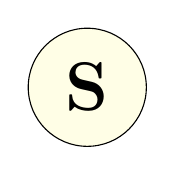
\begin{tikzpicture}
  \node[draw, circle, fill=yellow!10, minimum size=1.5cm, font=\bfseries\Huge] {S};
\end{tikzpicture}
\textit{“Is a breakthrough coming?”}
\end{center}
\end{tcolorbox}

Sometimes the perspectives Pixel has built clash so violently that
\textbf{something entirely new} emerges – a creative breakthrough no
one could have predicted.  Layer~13 listens for the first tremors of
such a knowledge earthquake.

\begin{tcolorbox}[colback=yellow!5, colframe=yellow!80, title=Real‑life analogy]
The invention of the steam engine didn’t just change transport; it
created a completely new understanding of work and energy.  Such leaps
appear sudden, but they were often preceded by years of building
tension.  Layer~13 recognises that build‑up.
\end{tcolorbox}

\textbf{Pixel feels the spark.}
Pixel sees an old concept about rock formations clashing with a new
idea about wind patterns.  The tension rises, and suddenly the system
snaps into a new state: a fresh, coherent theory that transcends both
ideas.  Pixel has discovered something no other system has ever thought
of.